%%%%%%%%%%%%%%%%%%%%%%%%%%%%%%%%%%%%%%%%%%%%%%%%
% This is the official Latex template prepared for the MSCS program at Weber State Universtiy
% This template is based on the Vanderbilt University Graduate School for submission of dissertations. 
% It is also based on a template originally prepared by Eli Hooten and updated by Haley Adams.

% Using the template is no guarantee that you pass format review with your first submission, but it should save you significant amount of time.

% This template is correct as of September 2021.
%%%%%%%%%%%%%%%%%%%%%%%%%%%%%%%%%%%%%%%%%%%%%%%%

\listfiles
\documentclass[10pt]{report}  %%% Changed from 12pt.

\usepackage[intoc]{nomencl}

\textwidth=6in \oddsidemargin=0.5in \topmargin=-0.5in
\textheight=9in  % 9in must include page numbers
\textfloatsep = 0.4in \addtocontents{toc}{\vspace{0.4in} \hfill
Page\endgraf} \addtocontents{lof}{\vspace{0.2in} \hspace{0.13in} \
Figure\hfill Page\endgraf} \addtocontents{lot}{\vspace{0.2in}
\hspace{0.13in} \ Table\hfill Page\endgraf}

% We've already imported some of the most commonly used packages for inserting formulas, images, tables, and references. If you need more, you can find a list of Latex packages here: https://www.ctan.org/pkg/ 

\usepackage{textcomp}
\usepackage{array}
\usepackage{listings}
\usepackage{setspace}
\usepackage{mathptmx}
\usepackage[table, svgnames]{xcolor}
\usepackage{colortbl}
\usepackage{graphicx}
\usepackage{amssymb, amsmath}
\usepackage{subfig}
\usepackage{epsfig}
\usepackage{times}
\usepackage{float}
\usepackage{rotating}
\usepackage{makeidx}
\usepackage{url}
\usepackage{multirow}
\usepackage{booktabs}
\usepackage{tabularx}
\usepackage{float}

\usepackage[subfigure, titles]{tocloft}
\usepackage{acronym}
\usepackage{datetime}
\usepackage[toc,page]{appendix}

%%another algorithm package
\usepackage{algorithm}
\usepackage{algorithmic}

\renewcommand{\nomname}{LIST OF ABBREVIATIONS}
\makenomenclature

\graphicspath{{Figures/}}
\DeclareGraphicsExtensions{.pdf,.jpeg,.png,.PNG, .eps, .tiff}


\usepackage{makecell}
\usepackage{titletoc}
\usepackage{sfchap}
\usepackage{sfsection}
\usepackage{cite}
\usepackage[numbers]{natbib}
%\usepackage[nottoc]{tocbibind}
%\usepackage[authoryear]{natbib}
%\usepackage{apacite}
\usepackage{appendix}
%\usepackage{tocbibind}

%
\setcounter{secnumdepth}{7}
\setcounter{tocdepth}{7}

\usepackage{hyperref}
\hypersetup{
    colorlinks=true,
    linkcolor=blue,
    filecolor=magenta,      
    urlcolor=cyan,
    pdftitle={Thesis Example},
    pdfpagemode=FullScreen,
}%
\urlstyle{same}

\usepackage[all]{hypcap}

% Stats table label
\newcommand{\statslabel}[2]{\multirowcell{#1}[-1.6mm][c]{#2}}

% Below heading rule.
\newcommand{\otoprule}{\midrule[\heavyrulewidth]}

% Prevent double spaced equations
\newenvironment{tightequation}{\singlespace\begin{equation}}{\end{equation}}

% Extra junk to pretty up the table of contents
\setlength{\cftsecnumwidth}{2.8em}
\setlength{\cftsubsecnumwidth}{3.7em}
\setlength{\cftsubsubsecnumwidth}{4.6em}
\setlength{\cftparanumwidth}{5.5em}
\setlength{\cftsubparanumwidth}{6.5em}
\setlength{\cfttabnumwidth}{3.5em}
\setlength{\cftfignumwidth}{3.5em} 

\renewcommand{\contentsname}{TABLE OF CONTENTS}
\renewcommand{\listfigurename}{LIST OF FIGURES}
\renewcommand{\listtablename}{LIST OF TABLES}
\renewcommand{\bibname}{ \texorpdfstring{{References\vspace{10mm}}}{References}   }
%
\renewcommand{\chaptermark}[1]{%
  \markboth{\MakeUppercase{%
      \chaptername}\ \thechapter.%
    \ #1}{}}
    
    
\interfootnotelinepenalty=10000 %prevents the splitting of long footnotes across multiple pages. Use with caution. 

\begin{document}

%%%%%%%%%%%%%%%%%%%%%%%%%%%%%%%%%%%%%%%%%%%%%%%%%%%%%%%%%%%%%%%%%%%%%%%%%%%%%%%%
%% Prevent the warning: pdfTeX warning (ext4): destination with the same identifier (name{page.1}) has been already used, duplicate ignored
%%	This setting will make a difference to the output because the page number is suppressed for the title page
\pagenumbering{alph}



 
\begin{titlepage}
\thispagestyle{empty}\enlargethispage{\the\footskip}%
\begin{center}
    \hspace{1em}\vspace{6em} \\ % add space before content
	{\setstretch{1.66} \MakeUppercase{Atmosniffer desktop application}\par }% TODO Change this
	\vskip.2in
	By
	\vskip .2in
	{Miguel Castrejon}   % TODO Change this
	\vskip .2in
	
	\begin{doublespace}
	A project report\\     % TODO Change this to project report OR thesis
		Submitted to the faculty of the \\ 
		MSCS Graduate Program of Weber State University\\
		in partial fulfillment of the requirements \\
		for the degree of \\ [.2in]
	\end{doublespace}
	
	MASTER OF SCIENCE \\[.1in]
	in \\[.1in]
	Computer Science \\[.1in]
	October 10, 2021 \\[.2in]  % TODO Change this
	%%%The date will reflect your proposed degree conferral date as selected from the Intent to Graduate form. This is your actual graduation date, not your thesis or defense date.%%%
	
	Ogden, Utah
	\vskip .5in
\end{center}


%%%Uncomment for Signatures%%%
\begin{doublespace}
Approved: \hskip 2.5in Date:\\[.2in]
\rule{3.5in}{.5pt} \hskip 0.1in \rule{2in}{.5pt} \\[.1in]
Hugo Valle, PhD. Committee chair. \\  [.2in]
\rule{3.5in}{.5pt} \hskip 0.1in \rule{2in}{.5pt} \\[.1in]
Yong Zhang, PhD. Committee member \\ [.2in]
\rule{3.5in}{.5pt} \hskip 0.1in \rule{2in}{.5pt} \\[.1in]
Abdulmalek Al-Gahmi, PhD. Committee member \\ [.2in]
%\rule{3.5in}{.5pt} \hskip 0.1in \rule{2in}{.5pt} %\\[.1in]
\end{doublespace}
%%%%%%%%%%%%%%

%%%%%%Uncomment  for Approved Names%%%%%%
%\begin{center}
%\begin{doublespace}
%Approved:\\ [.2in]
%Committee Chair, Ph.D. \\  [.1in]
%Committee member, Ph.D. \\ [.1in]
%Committee member, Ph.D. \\ [.1in]
%Committee member, Ph.D.
%\end{doublespace}
%\end{center}

\end{titlepage}

%%%%%%%%%%%%%%%%%%%%%%%%%%%%%%%%%%%%%%%%%%%%%%%%%%%%%%%%%%%%%%%%%%%%%%%%%%%%%%%%
\doublespacing
\pagenumbering{roman} \setcounter{page}{2}

% These 3 sections are optional 
\singlespacing  
%\doublespacing % Single or Double spacing for these sections?
%

\chapter*{}
\hspace{1em}\vspace{18em} \\ % add space before content
\begin{center}
    Copyright {\textcopyright} 2021 Miguel Castrejon \\
    All Rights Reserved     
\end{center}



%\input{Sections/Dedication}
%\input{Sections/Acknowledgments}
%\input{Sections/Abstract}


%%%%%%%%%%%%%%%%%%%%%%%%%%%%%%%%%%%%%%%%%%%%%%%%%%%%%%%%%%%%%%%%%%%%%%%%%%%%%%%%
\singlespacing
\tableofcontents

%%%%%%%%%%%%%%%%%%%%%%%%%%%%%%%%%%%%%%%%%%%%%%%%%%%%%%%%%%%%%%%%%%%%%%%%%%%%%%%%
\begingroup
\setlength{\parskip}{1\baselineskip}
%\listoftables
\newpage
\listoffigures
\newpage
%\printnomenclature %list of abbreviations is optional
%\newpage
\endgroup

%%%%%%%%%%%%%%%%%%%%%%%%%%%%%%%%%%%%%%%%%%%%%%%%%%%%%%%%%%%%%%%%%%%%%%%%%%%%%%%%
\normalsize
\doublespacing
\pagenumbering{arabic}
\setcounter{page}{1}

%Sections
\chapter{Atmosniffer Overview} %\label{Atmosniffer Overview}
%\vspace{-7mm}
%\bigskip
This Chapter provides an overview of the device the resarch team at Weber State University, led by Dr. Sohl and Dr. Valle started working on, the AtmoSniffer.

\section{Motivation}

\subsection{Why build a device that can "Sniff" the atmosphore?}
- “An estimated 4.2 million premature deaths globally are linked to ambient air pollution” according to the World Health Organization \cite{who}. In other words, the equivalent to the entire population of Utah every 9 months dies prematurely because of bad air. WHO estimates that 91\% of the world’s population is living in places where air quality guidelines are not met.\cite{who} Measuring this pollution is the first step in understanding and solving the problem. 


\begin{itemize}
\item \textbf{Problem:}
	\begin{itemize}
	\item Current air monitoring systems can be very large, heavy, and/or expensive
	\item They posses a limited range of sensors typically measuring only one gas type
	\item Are only usable for a specific task or deployment
	\item Require significant AC power.
	\end{itemize}

\item \textbf{Solution:}
	\begin{itemize}
	\item The AtmoSniffer is small and light.
	\item Detects a variety of gas types.
	\item Multiple user interfaces that can be easily accessed.
	\end{itemize}

\end{itemize}

\subsection{AtmoSniffer Project}
\begin{itemize}
\item The research team at Weber State University, led by Dr. Sohl and Dr. Valle started working on a device which is capable of moving air particles through gas sensors and transmit its data through radio and Bluetooth signals to monitor air quality and measure pollution. \cite{weber}

\item The current AtmoSniffer prototype, version 0.3, detects CO, CO2, NO, NO2, SO2, NH3, O3, VOCs, fine particulate material (in six size ranges covering 0.3 µm to 10 µm diameter aerosols), temperature, pressure, relative humidity, and inertial/true position. As a complete environmental monitor, turbulence/vibration is detected through a 9-axis inertial sensor. \cite{weber}

\item The AtmoSniffer can be deployed as a portable emissions locator or as a long duration air quality monitor staged on a work bench or mounted to pretty much anything.
\end{itemize}

\subsection{AtmoSniffer Device Pictures}
Here are a couple of pictures showing you how the physical device looks like:

\begin{figure}[h]
\centering
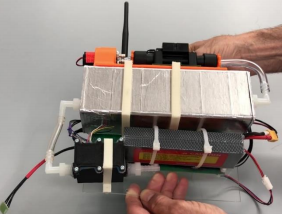
\includegraphics{full_device_cover.png}
 \caption{AtmoSniffer Device Encased, this is how the whole device looks when its assembled. \cite{weber}}
 \label{fig:encased_device}
\end{figure}

\begin{figure}[h]
\centering
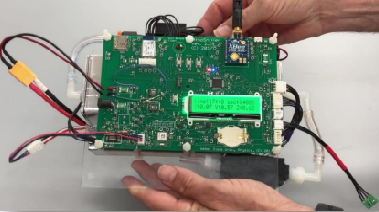
\includegraphics{full_device_nocover.png}
 \caption{Inside AtmoSniffer Device \cite{weber})}
 \label{fig:inside_device}
\end{figure}

\begin{figure}[h]
\centering
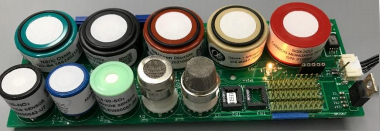
\includegraphics{gas_module.png}
 \caption{This is the Gas Sensors Module, this can be taken on/off like any other module.\cite{weber}}
 \label{fig:gas_sensors}
\end{figure}

\begin{figure}[h]
\centering
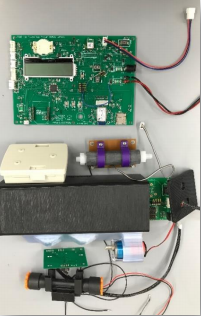
\includegraphics{modules_separated.png}
 \caption{Device Modules \cite{weber})}
 \label{fig:device_modules}
\end{figure}

\newpage \subsection{Project Interaces}
\begin{itemize}
\item The device transmits a stream of data via the following communication protocols:
	\begin{itemize}
	\item Xbee radio via UART channel; Fully functional
	\item Bluetooth via UART channel: Fully functional
	\item WIFI via UART Channel: To be develop
	\end{itemize}
\item Supports two Atmosniffer interfaces
	\begin{itemize}
	\item Android App
		\begin{itemize}
		\item Quick Diagnostic
		\item Data Calibration
		\end{itemize}
	\item Desktop Application
		\begin{itemize}
		\item Full Data Analysis
		\item Data Calibration
		\end{itemize}
	\end{itemize}
\end{itemize}

\chapter{MSCS Project Proposal} %\label{Atmosniffer Overview}
%\vspace{-7mm}
%\bigskip
This chapter provides the purpose, approach, research, and criteria on the approved project proposal.
\section{Purpose}
The main purpose of this application was to make a more user friendly AtmoSniffer Device Interface that could be easily accessed by both, developers and users.
Moreover, the main audience for the application is the research team at WSU. For them to be able to visualize data sent by a device, in a graph format, and to communicate and control the device for calibration purposes.

Other than building an application that people can easily use, I wanted to learn python, a new framework, such as qt, and how to professionally document a project.

\section{Approach}
To develop the application, I went through each step of the Software Development Life Cycle. With the help and permission of Dr. Valle, I created a GitHub repository to hold a copy of the old desktop application and start building from there. At first, I tried continuing and building up from the old desktop application, but I rather quickly found out that the old project lacked proper documentation and it was a much better idea to start from scratch rather than spend a whole month trying to decyphering it. I still kept the old project there under a legacy folder as a reference.

I was able to create a GUI and test it only with the help of python libraries. I met with users throughout and scheduled sprints to develop features.
\section{Research}
Research was focused on learning a QT, a new framework, and python. I used pyqt5 library which is the binding between qt and python.

The application needed to be able to handle a lot of data quickly. Python came with a big number of libraries used for data visualization, analysis, and parsing. This is the reason we chose it, but also because I have always wanted to learn it.

One more reason I found to do this project was for me to learn and experience a professional approach to software development. Including clean code, documentation, life cycle, testing, and a lot of messing up and debugging. 

The optimal goal of this project is to visualize a large amount of data.

\section{Criteria}
Application goals and milestones
\begin{itemize}
	\item Read data from SD card
	\item Visualize data from SD files
	\item Suppport bluetooth and radio connectivity.
		\begin{itemize}
		\item Connec to device
		\item Receive data from a device through bluetooth and/or radio signals
		\end{itemize}
	\item Visualize data from broadcast records.
		\begin{itemize}
		\item Create and close graphs
		\item Give the user the option to choose which type of graph they would like to see.
		\end{itemize}	
	\item Send commands to the connected device through bluetooth and/or radio signals
		\begin{itemize}
		\item Turn ON/OFF device components
		\item Enable extra debugging
		\item Reset sensors
		\end{itemize}
	\item Documentation
		\begin{itemize}
		\item Full documentation of code, following best standards.
		\item Documentation on how to use the application
		\end{itemize}
	\item Unit Testing
		\begin{itemize}
		\item This includes code and gui components of the application
		\end{itemize}
	\item Support Multiple OS
		\begin{itemize}
		\item Create executables/installers for various OS
		\end{itemize}
\end{itemize}

\chapter{AtmoSniffer Desktop Application} %\label{Atmosniffer Overview}
%\vspace{-7mm}
%\bigskip
This chapter provides an overview on the main differences between the old and new desktop application

\section{Old Desktop Application}
\begin{itemize}
\item The old "Desktop app" was very basic application, only used for debugging purposes.
	\begin{itemize}
	\item It connected to a single device
	\item Parsed data stream from radio signals
	\item Basic plotting of data members
	\item Basic I/O with device
	\item It was only able to be ran through a set of options from a terminal, no gui interface.
	\end{itemize}
\end{itemize}

\section{New Desktop Application}
\begin{itemize}
\item The proposed "Desktop app" was very basic application, only used for debugging purposes.
	\begin{itemize}
	\item Its able to connect and listen to multiple devices
	\item Parses data stream from both radio and bluetooth signals
	\item More advance plotting of data members, with the option to run different types of graphs.
	\item More advance and user friendly I/O with connected devices, using dropdown menu and textboxes.
	\item GUI interface for easier user navigation.
	\end{itemize}
\end{itemize}
\chapter{AtmoSniffer User Manual} %\label{Atmosniffer Overview}
%\vspace{-7mm}
%\bigskip
	Hello and welcome to the Desktop application for the AtmoSniffer!
	Here you will find all you need to know to install, run, and even develop the application.

	With this application you are able to coonnect to an atmosniffer device, open static report files, and compare data with the help of graphs. You are also able to communicate with the connected devices through commands. This is a python project, so please familiarize yourself with python first.
\section{Users}
Let's first start with a quick guide for every day users!
\subsection{Installation}
	For the every day user we have a very simple and easy to use installer, here is the link [], download and follow all instructions inside.
\subsection{Opening a file}
	So you want to look at old data and compare it with other device's or even the same device's data? Well you can do it by first making sure you have the desktop application running.
\begin{figure}[H]
\centering
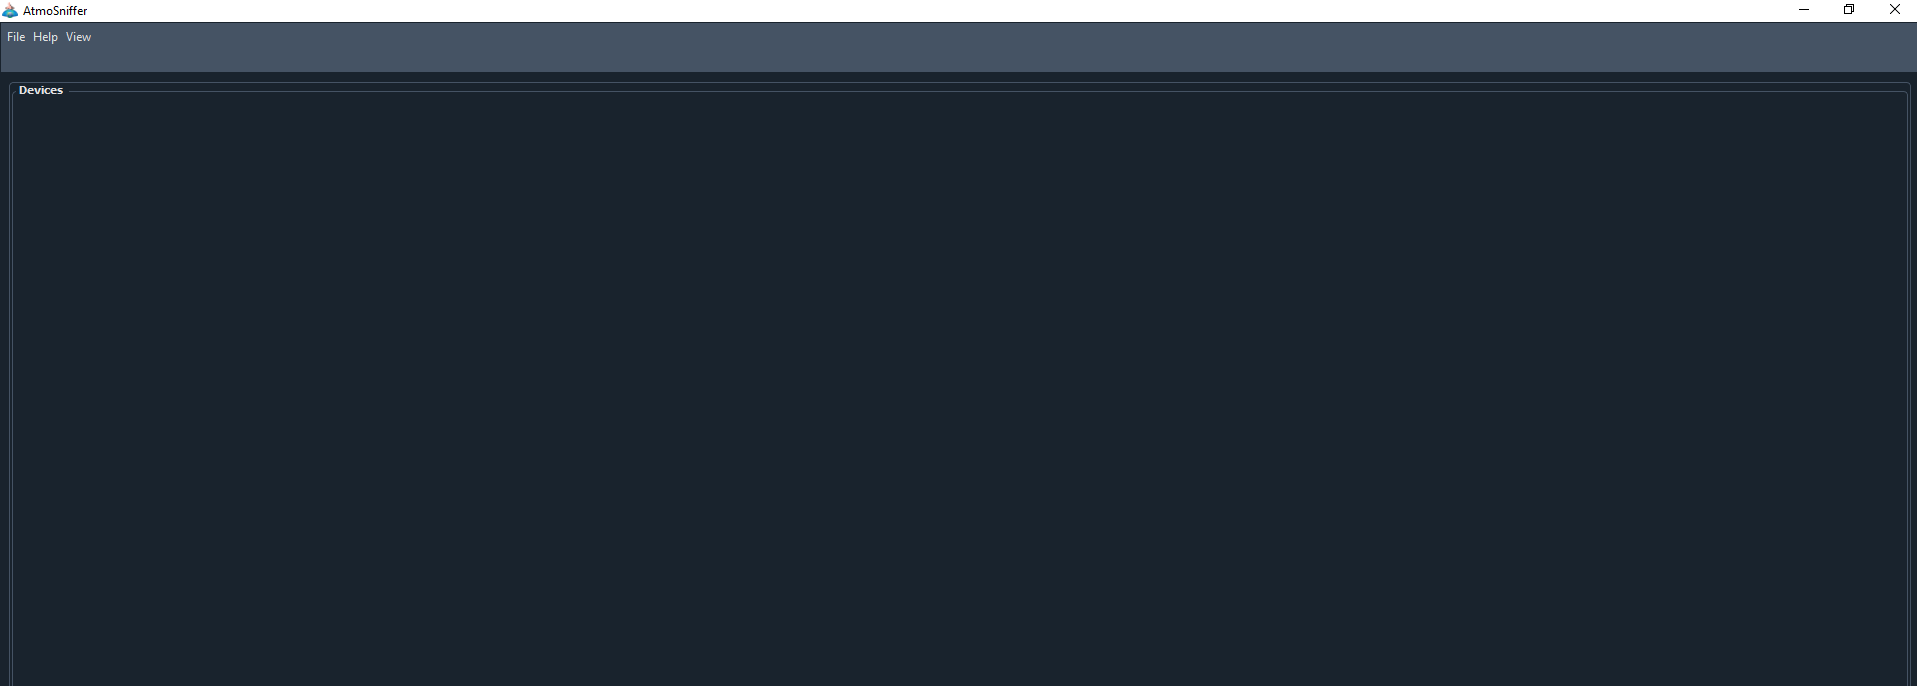
\includegraphics[width=15cm]{project_images/main_window.png}
 \caption{Main desktop window}
 \label{fig:main window}
\end{figure}
\newpage

	Use the menu item File on the left-top corner of the screen and then click Open. This should bring up a dialog for you to find whichever data file you would like to look at.

\begin{figure}[H]
\centering
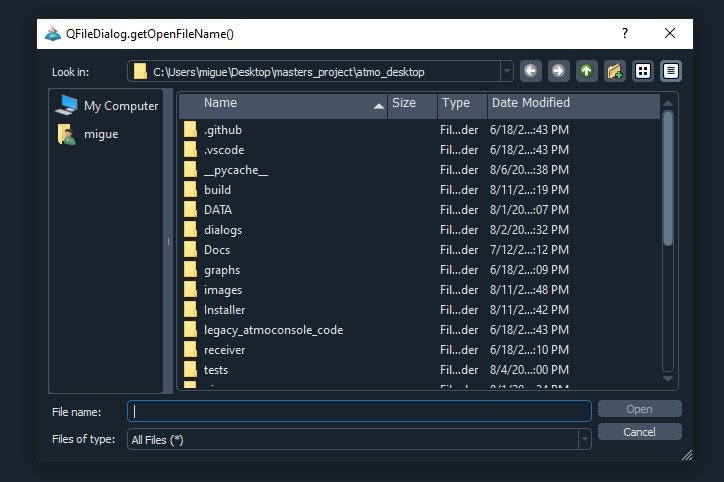
\includegraphics[width=9cm]{project_images/open_file_dialog.png}
 \caption{Open file dialog}
 \label{fig:open file dialog}
\end{figure}

	!You can also use the shortcut CTRL+O!

	After the dialog has popped up, navigate into the DATA folder and select your desired file, click okay and you should hopefully have a new device added into the application for analysis.

\begin{figure}[H]
\centering
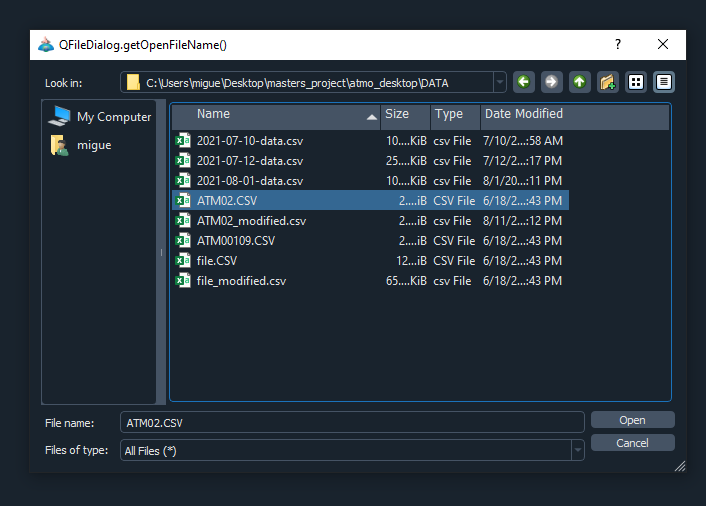
\includegraphics[width=9cm]{project_images/open_file_dialog_data_selection.png}
 \caption{Choosing ATM02.CSV from open file dialog}
 \label{fig:open file dialog data selection}
\end{figure}

	In this case we are using the ATM02.CSV file.

\begin{figure}[H]
\centering
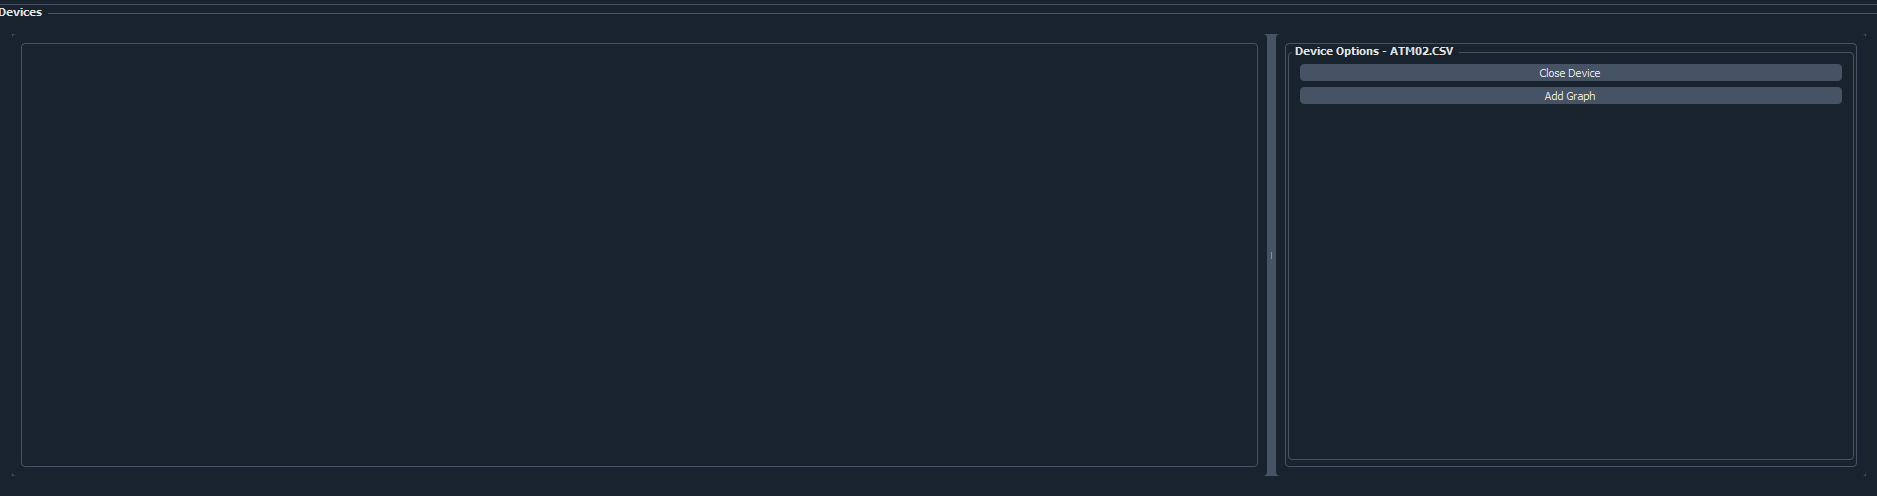
\includegraphics[width=15cm]{project_images/opened_device.png}
 \caption{ATM02.CSV file opened}
 \label{fig:opened atm02 csv file}
\end{figure}

\subsection{Adding a graph to an open file}
	Now that you have succesfully opened a device, lets try to add a graph to the main window and start analysing. First you will need to click the Add Graph button on the right side of the device and this next dialong should pop up.

\begin{figure}[H]
\centering
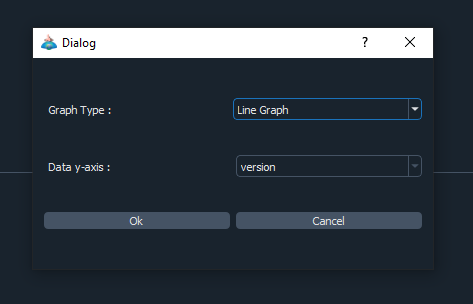
\includegraphics[width=9cm]{project_images/graph_dialog.png}
 \caption{Graph Dialog}
 \label{fig:graph dialog}
\end{figure}

	From here, go ahead and select wich type of graph you would like to see and then continue to select which x-axis/y-axis data item would you like to see. Please keep in mind that line graph and bar graph only need the x - axis item, but the scatter plot needs both. Once you have selected your desired graph type and items go ahead and click 'Ok'

\begin{figure}[H]
\centering
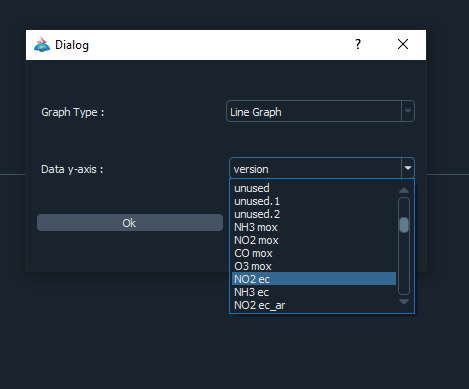
\includegraphics[width=9cm]{project_images/graph_dialog_select.png}
 \caption{Graph Dialog Selections}
 \label{fig:graph dialog selections}
\end{figure}

	This should add a new graph tab to our device window.

\begin{figure}[H]
\centering
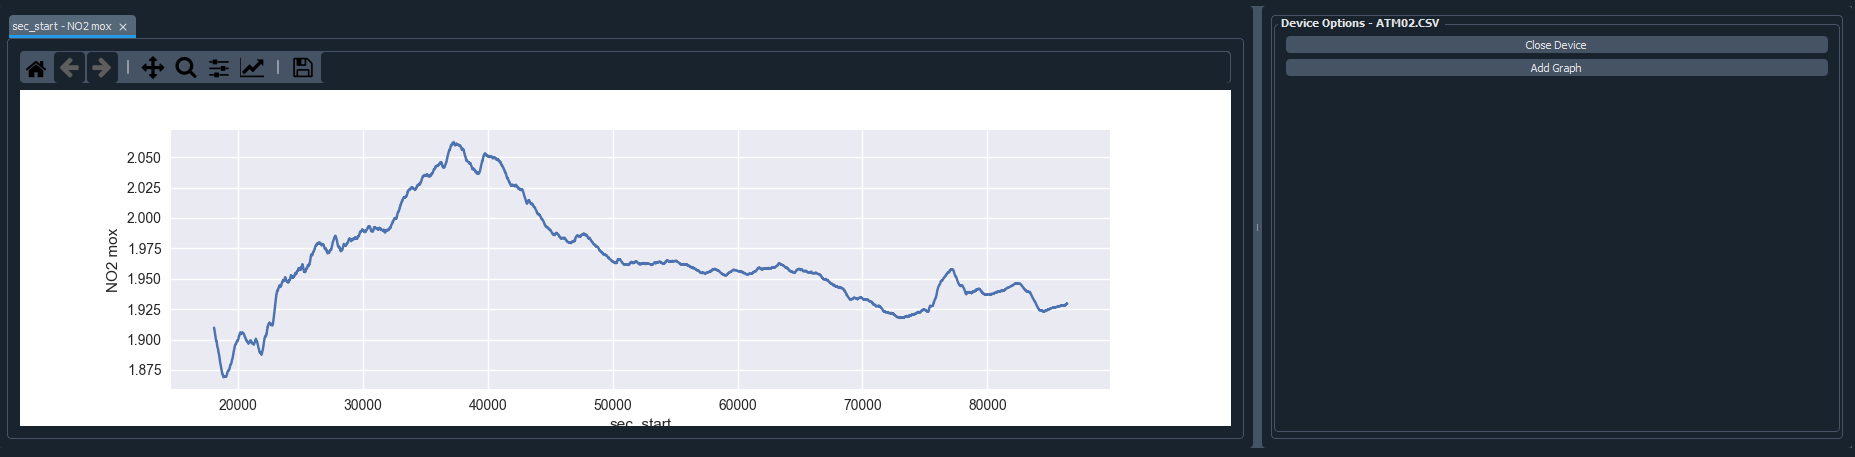
\includegraphics[width=15cm]{project_images/opened_graph_static_device.png}
 \caption{Opened graph on a static device, csv file}
 \label{fig:opened graph on static device}
\end{figure}

\subsection{Closing graphs}
	If you would like to close an opened graph, you just need to click on the small 'x' by the selected graph's tab.

\begin{figure}[H]
\centering
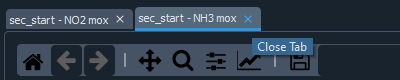
\includegraphics[width=9cm]{project_images/close_graph_icon.png}
 \caption{Close a graph}
 \label{fig:close a graph}
\end{figure}

\subsection{Connecting to an AtmoSniffer Device}
	If you would like to watch the data being transmitted from an AtmoSniffer device then all you have to do is go to the main window, go to the top left menu 'File', and then click Connect Device. This should bring up a little dialog window asking you to choose from the currently connected devices in your computer. This can be done through bluetooth or radio for now.
You can also use the shortcut CTRL+O!

\begin{figure}[H]
\centering
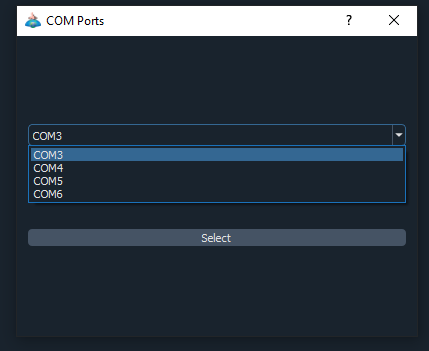
\includegraphics[width=9cm]{project_images/com_ports_dialog.png}
 \caption{Communication Ports Dialog}
 \label{fig:com ports dialog}
\end{figure}

	The image above shows the current connected devices on my computer, by going into the communication ports settings on my computer I know that I should be connecting to COM6 since that's what corresponds to the actual AtmoSniffer Device. I'll choose it from the dropdown menu and then proceed to click Select. If everything goes right we should get an additional outline added to our main window with the name of its corresponding communication port.

\begin{figure}[H]
\centering
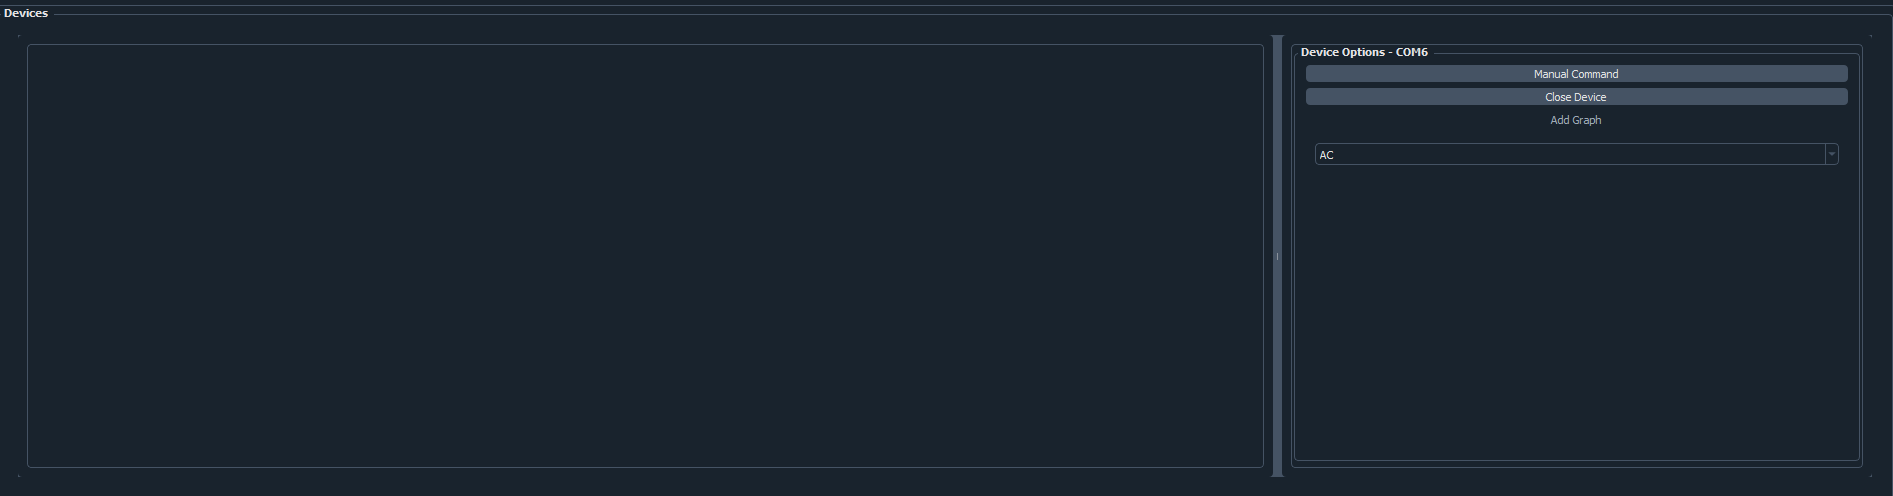
\includegraphics[width=15cm]{project_images/com_device_opened.png}
 \caption{Communication port device opened}
 \label{fig:com device opened}
\end{figure}

	Caution! Might sometimes not work as expected because of signals being sent through the 'air'

\begin{figure}[H]
\centering
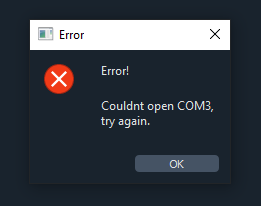
\includegraphics[width=9cm]{project_images/error_com_dialog.png}
 \caption{Error dialog for communication port}
 \label{fig:com port error}
\end{figure}

	If this happens, it can mean one of two things. It could be that you are trying to connect to a communication port that does not correspond to an AtmoSniffer Device or it just had a small hiccup and you should just try again.

\subsection{Sending commands to connected device}

	Before you are able to send any commands, please make sure you have succesfully connected to a device first and then follow either one of the next list items.
	By clicking on 'View' -> 'Terminal' a terminal window will be added to the bottom of the screen and you will be able to see the commands being sent to the connected device.

	\begin{itemize}
	\item Manual:
	\newline To be able to send a command manually, click on the device's 'Manual Command' button, this should pop up a window.

	\begin{figure}[H]
	\centering
	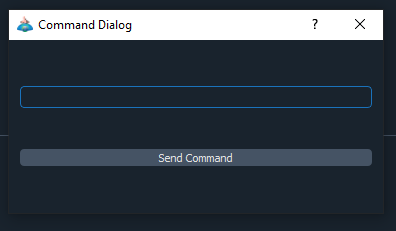
\includegraphics[width=9cm]{project_images/manual_command_dialog.png}
	 \caption{Manual command dialog}
	 \label{fig:manual command dialog}
	\end{figure}

	Now go ahead and type in your command and then proceed to press 'Send Command', in this case I will be sending 'ac 0', which should turn it off.

	\begin{figure}[H]
	\centering
	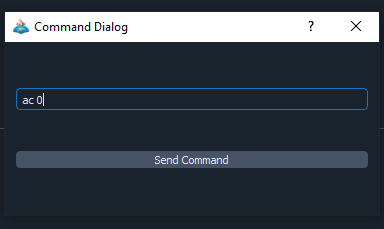
\includegraphics[width=9cm]{project_images/command_dialog_ac.png}
	 \caption{Turning off the ac module through a manual command}
	 \label{fig:manual command ac}
	\end{figure}

	\item Dropdown Menu:
	\newline Using the dropdown menu can sometimes speed things up since you won't be needing to type anything down.
	
	\begin{figure}[H]
	\centering
	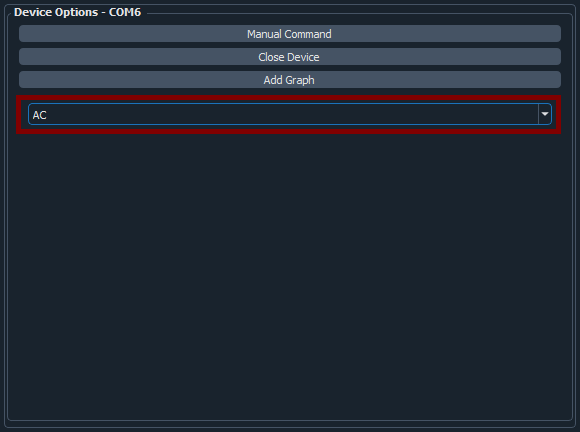
\includegraphics[width=9cm]{project_images/dropdown_menu_dynamic_device.png}
	 \caption{Dynamic device, dropdown menu}
	 \label{fig:dropdown menu dynamic device}
	\end{figure}

	Just click on the name of the module you would like to interact with and click on one of it's pre configured options.

	\begin{figure}[H]
	\centering
	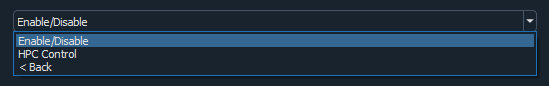
\includegraphics[width=9cm]{project_images/dropdown_menu_command_options.png}
	 \caption{Dropdown menu command options}
	 \label{fig:dropdown menu command options}
	\end{figure}
	\end{itemize}

	\subsection{Closing a connected device}
	Now you are all set up and are able to enjoy the application! To close a device, just click on the 'Close Device' button and you are set!

	\begin{figure}[H]
	\centering
	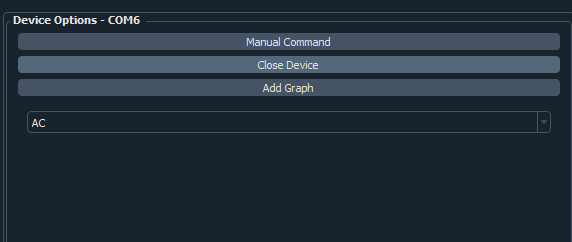
\includegraphics[width=9cm]{project_images/dy_close_device_button.png}
	 \caption{Close dynamic device}
	 \label{fig:close dynamic device}
	\end{figure}
	

\newpage
\section{Developers}
\subsection{Installation}
\begin{itemize}
\item Installer
\newline As a developer I think the Installer is not your best option, but why not, right? Just follow the installer instructions as you download it here link...
\item Required libraries
\newline First, you will need to clone this repository into your local branches. Then, inside the Docs folder there is a file with the name 'requirements.txt' this file contains the name of all libraries used in this application. This is very useful because we can use the command 'pip install -r requirements'.txt to download and install them all.

\begin{figure}[H]
\centering

\includegraphics[width=9cm]{project_images/pip_install_requirements.png}
 \caption{Installing requirements with pip}
 \label{fig:pip install requirements}
\end{figure}

In my case, I have all those libraries installed already so I get a bunch of 'Requirement already satisfied' messages.

\begin{figure}[H]
\centering
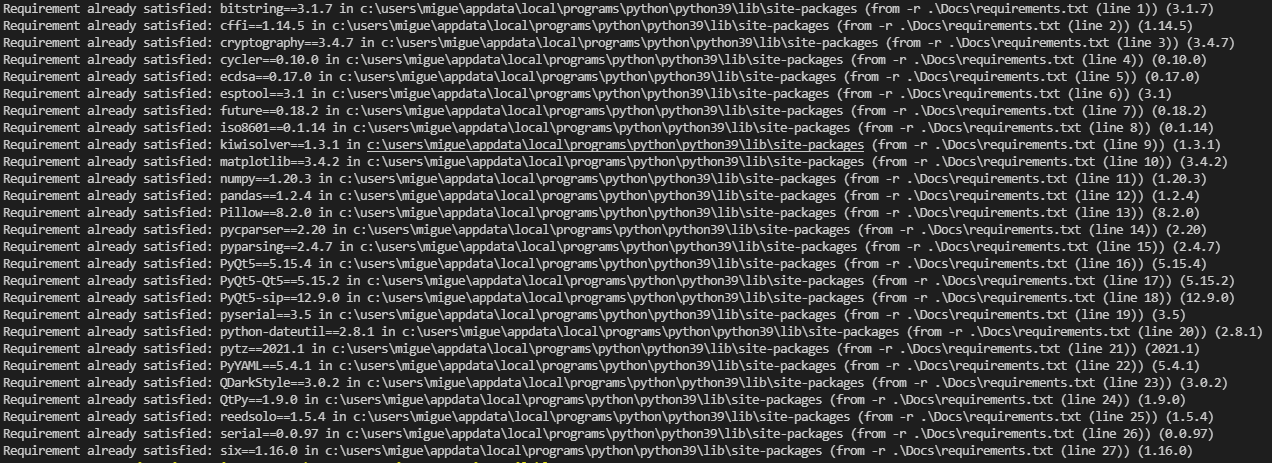
\includegraphics[width=12cm]{project_images/requirements_satisfied.png}
 \caption{Requirements satisfied}
 \label{fig:requirements satisfied}
\end{figure}

If you have added a new library into the application, use the command 'pip freeze > ./Docs/requirements.txt' in the main folder and it should create a new 'requirements.txt' file that can be later used to install all required libraries.

\begin{figure}[H]
\centering

\includegraphics[width=9cm]{project_images/pip_freeze.png}
 \caption{Pip freeze}
 \label{fig:pip freeze}
\end{figure}	
\end{itemize}

\subsection{Creating the installer}
	For this project, I use cx$\_$Freeze and InnoSetup to make an executable and the installer, it is fairly easy to make. I have already made a python file called setup.py which can be called with the command 'py setup.py build', this will run it and create an executable inside the folder build.

\begin{figure}[H]
\centering

\includegraphics[width=4cm]{project_images/setup_build.png}
 \caption{Setup command}
 \label{fig:setup command}
\end{figure}	

\begin{figure}[H]
\centering
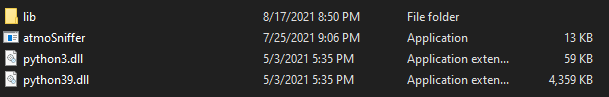
\includegraphics[width=9cm]{project_images/build_folder.png}
 \caption{Build folder}
 \label{fig:build folder}
\end{figure}	
	
	Once the executable has been created you will notice that it won't really work, this is because once the executable is created it does not move all required files into the build folder. Here is where we come in, we have to move in all dependencies into the build folder. All folders and files such as; receiver, ui, images, graphs, dialogs, DATA, com$\_$popup.py, Device.py, etc. Once this is done, try running the executable, if it works then we can move on to making the installer.

\begin{figure}[H]
\centering
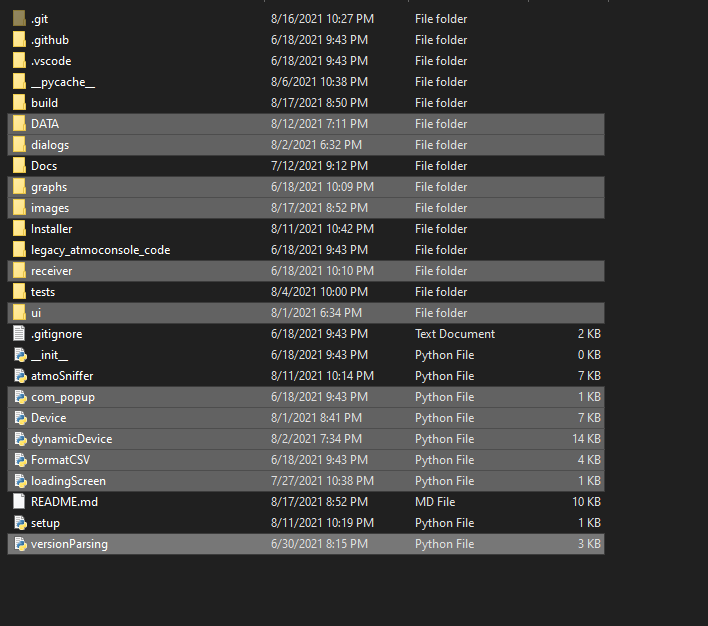
\includegraphics[width=9cm]{project_images/required_files.png}
 \caption{Required files for executable to work}
 \label{fig:required files}
\end{figure}	

\begin{figure}[H]
\centering
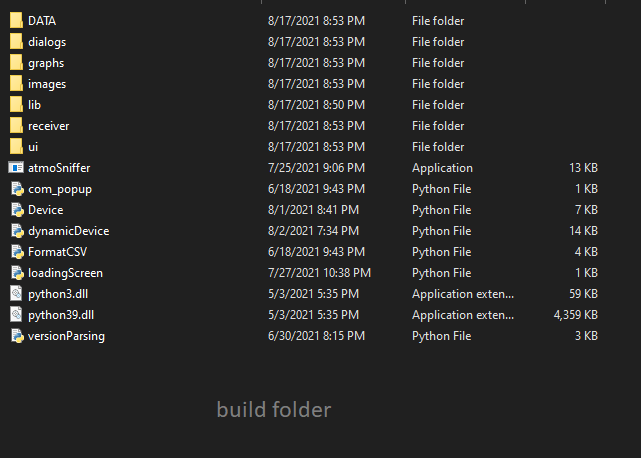
\includegraphics[width=9cm]{project_images/build_folder_required.png}
 \caption{Inside build folder with required files}
 \label{fig:required files in build folder}
\end{figure}	

	So I like I had said before, I use InnoSetup, it is fairly easy to use. I'm currently using their 6.2.0 version. You can download it from THIS LINK (https://jrsoftware.org/isdl.php).
	After running InnoSetup, you will get this Welcome dialog. Choose "Create a new script file using the Script Wizard" and click "Ok".

\begin{figure}[H]
\centering
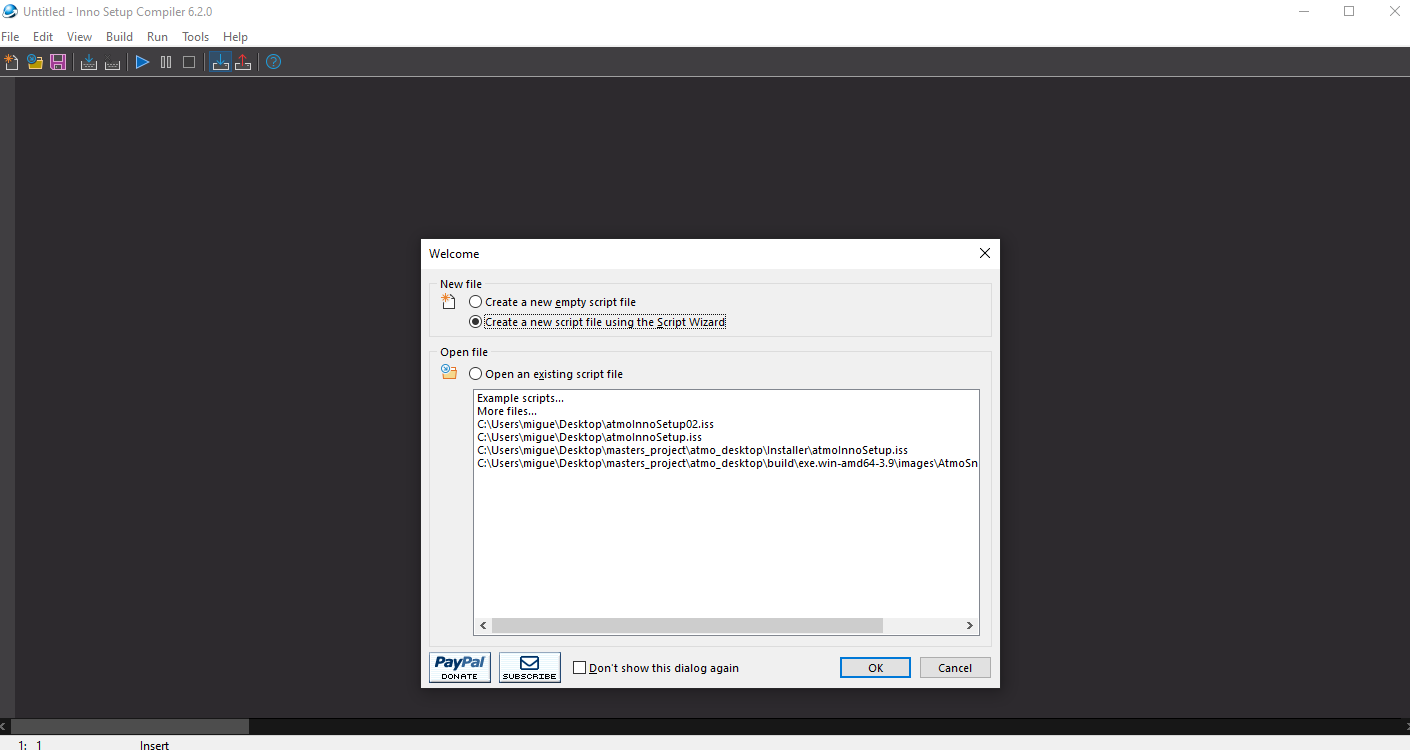
\includegraphics[width=9cm]{project_images/inno_setup_welcome.png}
 \caption{Using Inno Setup to make an installer}
 \label{fig:inno setup welcome}
\end{figure}

	Click "Next" on the next popup window, until you get to this window where we need to fill in our application information.

\begin{figure}[H]
\centering
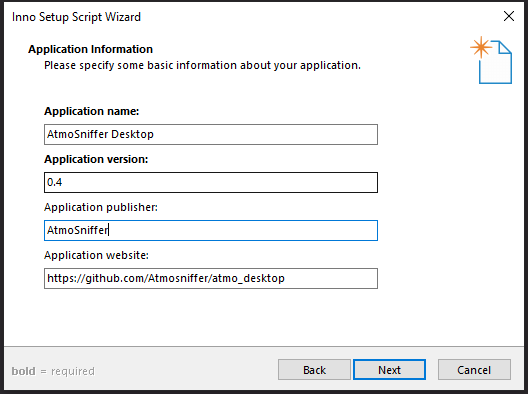
\includegraphics[width=9cm]{project_images/inno_atmo_info.png}
 \caption{Information concerning our application}
 \label{fig:inno atmo info}
\end{figure}

	Next we will continue to press "Next" until we find ourselves in the Application Files Window, where we need to add all of the files in our "build" folder by clicking "Add File(s)" and/or "Add Folder"

\begin{figure}[H]
\centering
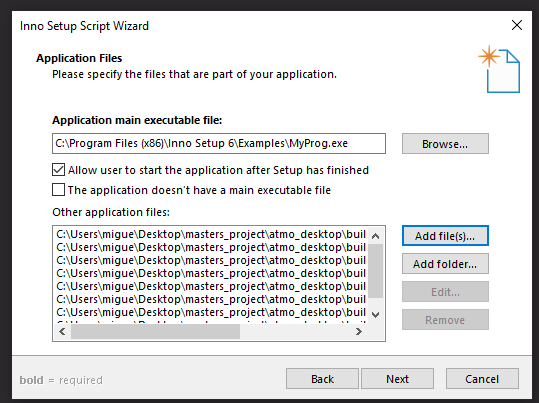
\includegraphics[width=9cm]{project_images/inno_added_files.png}
 \caption{Adding files to the installer}
 \label{fig:inno added files}
\end{figure}

\begin{figure}[H]
\centering
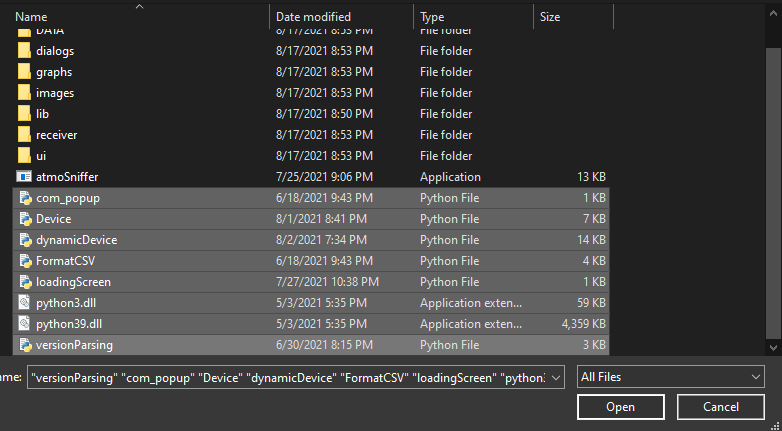
\includegraphics[width=9cm]{project_images/inno_selected_files.png}
 \caption{Selected files in Inno Setup}
 \label{fig:inno selected files}
\end{figure}
	
	It is a little different for adding folders, first we choose which folder we would like to add and then we select it and click on the "Edit" button to make sure our folder contents are added to the right folder inside our application's installation folder

\begin{figure}[H]
\centering
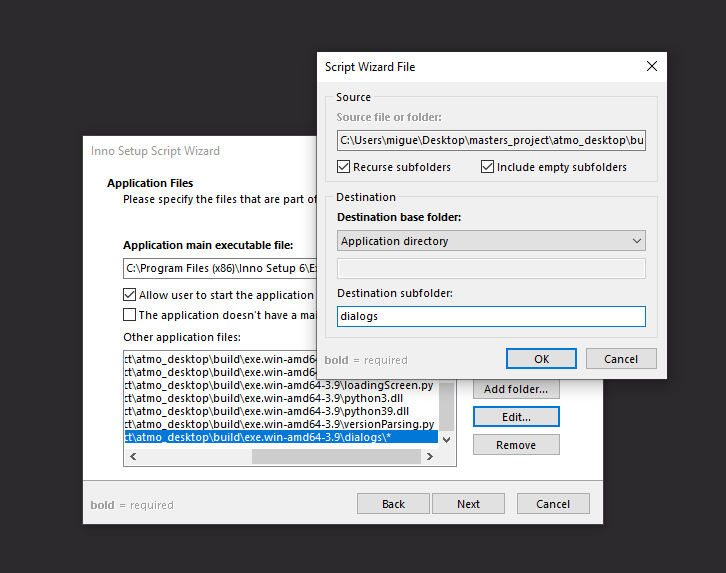
\includegraphics[width=9cm]{project_images/inno_adding_folder.png}
 \caption{Adding folders to inno setup}
 \label{fig:inno adding folder}
\end{figure}

	In the image above, you can see that for the folder dialogs, you need to click on it, edit it and add the string "dialogs" under "Destination subfolder", and then click "Ok". Do this for all folders inside the build folder.

	Do not include the .exe under "Other application files"

	At last, we should select our executable file with the "Browse" button in the "Application Files" window.

\begin{figure}[H]
\centering
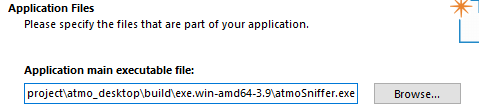
\includegraphics[width=9cm]{project_images/inno_added_exe.png}
 \caption{Selecting the exe file}
 \label{fig:inno added exe}
\end{figure}

	Next, we continue clicking "Next" until we get to the "Compiler Settings" window where we are going to set our output file name, and choose the icon file from the build/images/ folder called logo$\_$icon.ico as the application's icon image.

\begin{figure}[H]
\centering
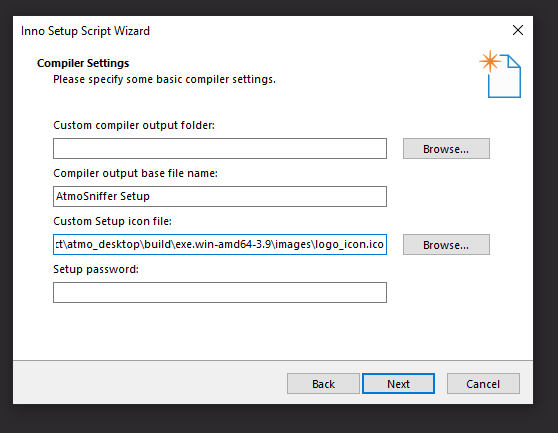
\includegraphics[width=9cm]{project_images/inno_compiler_window.png}
 \caption{Choosing compiler inno setup}
 \label{fig:inno compiler window}
\end{figure}

	After you have something like the image above, click next until you see the finish button and click on it. Next up you will be asked if you want to run the script. Click on "No".
	You will see something like this:

\begin{figure}[H]
\centering
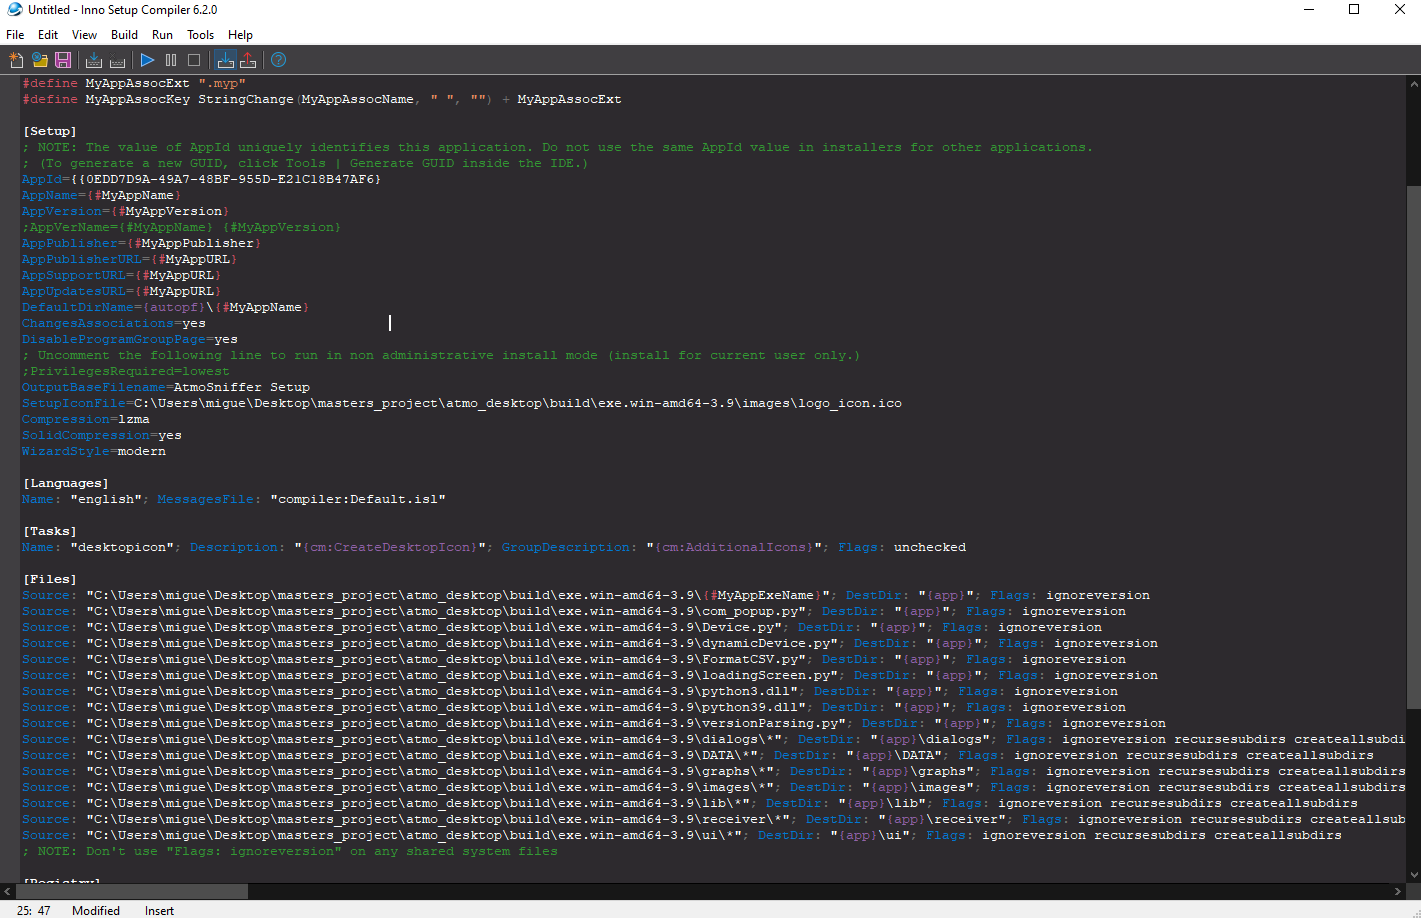
\includegraphics[width=15cm]{project_images/inno_atmo_script.png}
 \caption{Inno Setup Script Example}
 \label{fig:inno atmo script}
\end{figure}

	From here, there are two things we need to ensure we do. First, we need to give our users persmission to modify the DATA folder since our computer software will not allow us to modify anything inside the "Program Files" folder without permissions. For this we need to look for our "DATA" folder source and add "; Permissions: users-modify"

\begin{figure}[H]
\centering
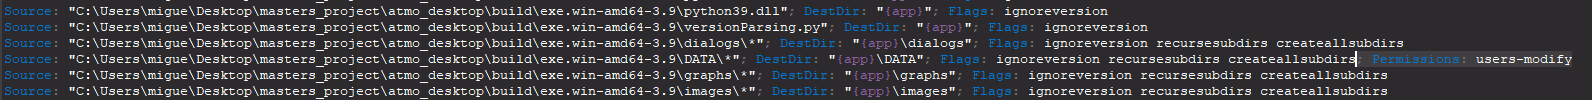
\includegraphics[width=15cm]{project_images/inno_users_modify.png}
 \caption{Giving users the required permissions to modify files in system folders}
 \label{fig:inno users modify}
\end{figure}

	Now that we have that solved, we need to make sure the icon will show correctly for the setup/installer and the executable. Lets move down the script until we see the "[Icons]" Group, here we will copy both items and paste them right under the other two.

\begin{figure}[H]
\centering
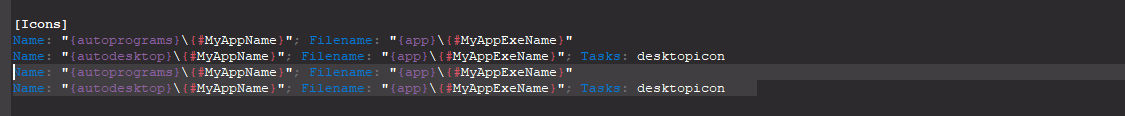
\includegraphics[width=15cm]{project_images/inno_icons_copy.png}
 \caption{Setting up placeholders for icons.}
 \label{fig:inno icons copy}
\end{figure}

	And we edit both copies with IconFilename:" \textbraceleft app\textbraceright 	\textbackslash images\textbackslash logo\_icon.ico" 

\begin{figure}[H]
\centering
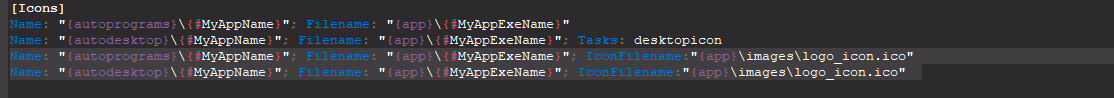
\includegraphics[width=15cm]{project_images/inno_icons_iconfilename.png}
 \caption{Editing script line to correctly use icons.}
 \label{fig:inno icons iconfilename}
\end{figure}

	Next, we save the script and run it. Once the script is done running you need to go to the folder where you saved your script at and look for the "Output" folder. It will contain our installation executable, which can then be used to install the AtmoSniffer Desktop application.

\begin{figure}[H]
\centering

\includegraphics[width=15cm]{project_images/atmo_setup_installer.png}
 \caption{Atmosniffer setup installer.}
 \label{fig:atmo setup installer}
\end{figure}

\subsection{Adding more commands to device command dropdown}
	We can use the AtmoSniffer Desktop application to communicate to connected "devices" this can be done by either, manually typing the command in a text box or by using a the custom dropdown embedded into a device widget. With the addition of new AtmoSniffer versions we could be getting new useful commands that would be much easier to use through the dropdown menu, rather than manually typing it in, but they haven't been added yet.

	If this happens we need to go to the dynamicDevice.py, here is where we can add new commands. At first we need to make a decision, do we want to add a new module to the whole program or do we just need to work on an existing module? If a new module is needed then we need to go to the self.cmd$\_$list.addItems() line and inside the function call we need to add the name of said module. Else, we just leave it how it is.

\begin{figure}[H]
\centering
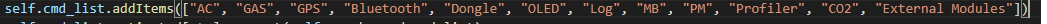
\includegraphics[width=15cm]{project_images/submenu_cmd_list.png}
 \caption{Submenu cmd list.}
 \label{fig:submenu cmd listr}
\end{figure}

	Now that that's done we go down to the on\_changed\_cmd\_list function where we will need to keep in mind which commands we will be sending to the selected module.

	Here is where it gets a bit tricky but don't worry I promise is not that hard. We are essentially building up a command inside a stack. The first "if" block checks for wether we have already started building a command or not. If not, then it will first add the module name to the command stack, "self.cmd". and change the dropdown menu with the new options for said module.

\begin{figure}[H]
\centering
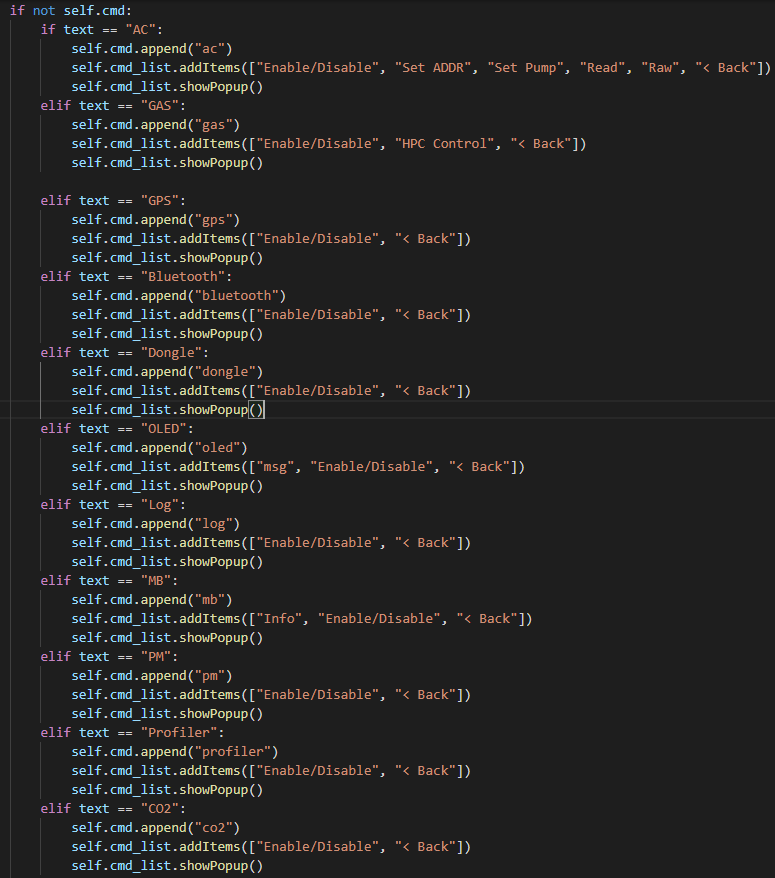
\includegraphics[width=13cm]{project_images/cmd_list_first_if.png}
 \caption{First if block in the command making process.}
 \label{fig:cmd list first if}
\end{figure}

	Next, we know that the option the user clicked on cannot be the first time they clicked so we check which option they clicked on, and depending on the first index of our command stack we change the command dropdown with new options, but not without checking if the first index module is supposed to have these new options first.
	We always want to append something to our stack even if its meaningless, otherwise the function will not work since it could remove the wrong item once the option \textless back is clicked, for this we add meaningless options surrounded by \textless and\textgreater.
	Once an end argument is reached, we add the end argument and the item \textless end\textgreater to our command stack
	For example if the option they clicked on is "Battery Volts" then we first check if the first index of the command stack has the word "mbi", if so we append a "4" and then the \textless end\textgreater tag.

\begin{figure}[H]
\centering
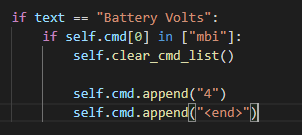
\includegraphics[width=9cm]{project_images/battery_volts_example.png}
 \caption{Battery volts command example.}
 \label{fig:battery volts example}
\end{figure}
	
	Lastly, we check if the command stack has the \textless end\textgreater tag, if so we build the command by first looking for all those meaningless tags and removing them, and then joining the remaining stack items into a single string and sending it to the device itself with a helper method.

\subsection{Add more headers for upcoming versions}

	At the time this guide is being created, AtmoSniffer has 2 versions; 2.0 and 3.0. The project will continue to grow which means that more versions will be added.
	For this, we need to make sure we tell the application about the new versions or it will continue to crash. This can be done by going to the file versionParsing.py

\begin{figure}[H]
\centering
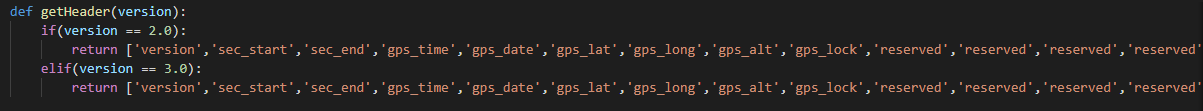
\includegraphics[width=15cm]{project_images/version_parsing.png}
 \caption{Version parsing.}
 \label{fig:version parsing}
\end{figure}

We just need to add a new elif statement with our new version number with the correct returned header. Keep the version number as a double/float.





\begin{appendices}
\chapter{Python Libraries used to develop the application} %\label{Python libraries}
%\vspace{-7mm}
%\bigskip
	Here is a list of all python libraries used in the developing of the atmosniffer desktop application:
\begin{itemize}
	\item pyqt5
		\\* PyQt5 is a comprehensive set of Python bindings for Qt v5. It is implemented as more than 35 extension modules and enables Python to be used as an alternative application development language to C++ on all supported platforms including iOS and Android.
		\\* https://pypi.org/project/PyQt5/
	\item serial
		\\*  A framework for serializing/deserializing JSON/YAML/XML into python class instances and vice versa
		\\* https://pypi.org/project/serial/
	\item webbrowser
		\\ The webbrowser module provides a high-level interface to allow displaying Web-based documents to users. Under most circumstances, simply calling the open() function from this module will do the right thing.
		\\* https://docs.python.org/3/library/webbrowser.html
	\item pandas
		\\* Powerful data structures for data analysis, time series, and statistics
		\\* https://pypi.org/project/pandas/
	\item csv
		\\* The csv module implements classes to read and write tabular data in CSV format. It allows programmers to say, “write this data in the format preferred by Excel,” or “read data from this file which was generated by Excel,” without knowing the precise details of the CSV format used by Excel. Programmers can also describe the CSV formats understood by other applications or define their own special-purpose CSV formats.
		\\* https://docs.python.org/3/library/csv.html
	\item os
		\\* This module provides a portable way of using operating system dependent functionality.
		\\* https://docs.python.org/3/library/os.html
	\item cx$\_$freeze
		\\* cx$\_$Freeze creates standalone executables from Python scripts, with the same performance, is cross-platform and should work on any platform that Python itself works on.
		\\* https://pypi.org/project/cx-Freeze/
	\item matplotlib
		\\* Matplotlib is a comprehensive library for creating static, animated, and interactive visualizations in Python.
		\\* https://pypi.org/project/matplotlib/
	\item io
		\\* The io module provides Python’s main facilities for dealing with various types of I/O.
		\\* https://docs.python.org/3/library/io.html
	\item datetime
		\\* The datetime module supplies classes for manipulating dates and times.
		\\* https://docs.python.org/3/library/datetime.html
\end{itemize}





\end{appendices}
%\chapter{Python Libraries used to develop the application} %\label{Python libraries}
%\vspace{-7mm}
%\bigskip
	Here is a list of all python libraries used in the developing of the atmosniffer desktop application:
\begin{itemize}
	\item pyqt5
		\\* PyQt5 is a comprehensive set of Python bindings for Qt v5. It is implemented as more than 35 extension modules and enables Python to be used as an alternative application development language to C++ on all supported platforms including iOS and Android.
		\\* https://pypi.org/project/PyQt5/
	\item serial
		\\*  A framework for serializing/deserializing JSON/YAML/XML into python class instances and vice versa
		\\* https://pypi.org/project/serial/
	\item webbrowser
		\\ The webbrowser module provides a high-level interface to allow displaying Web-based documents to users. Under most circumstances, simply calling the open() function from this module will do the right thing.
		\\* https://docs.python.org/3/library/webbrowser.html
	\item pandas
		\\* Powerful data structures for data analysis, time series, and statistics
		\\* https://pypi.org/project/pandas/
	\item csv
		\\* The csv module implements classes to read and write tabular data in CSV format. It allows programmers to say, “write this data in the format preferred by Excel,” or “read data from this file which was generated by Excel,” without knowing the precise details of the CSV format used by Excel. Programmers can also describe the CSV formats understood by other applications or define their own special-purpose CSV formats.
		\\* https://docs.python.org/3/library/csv.html
	\item os
		\\* This module provides a portable way of using operating system dependent functionality.
		\\* https://docs.python.org/3/library/os.html
	\item cx$\_$freeze
		\\* cx$\_$Freeze creates standalone executables from Python scripts, with the same performance, is cross-platform and should work on any platform that Python itself works on.
		\\* https://pypi.org/project/cx-Freeze/
	\item matplotlib
		\\* Matplotlib is a comprehensive library for creating static, animated, and interactive visualizations in Python.
		\\* https://pypi.org/project/matplotlib/
	\item io
		\\* The io module provides Python’s main facilities for dealing with various types of I/O.
		\\* https://docs.python.org/3/library/io.html
	\item datetime
		\\* The datetime module supplies classes for manipulating dates and times.
		\\* https://docs.python.org/3/library/datetime.html
\end{itemize}





%\chapter{References} %\label{References}
%\vspace{-7mm}
%\bigskip

\begin{itemize}
	\item Sohl, J.E. et al. (2019) 'The Atmosniffer: A Broad Spectrum, Air $\&$ Enverionmental Monitoring System', Business Plan.
	\item https://www.who.int/news-room/fact-sheets/detail/ambient-(outdoor)-air-quality-and-health (Accessed on May 30, 2019) 
\end{itemize}
%\input{Sections/Chapter1}
%\input{Sections/Chapter2}
%\input{Sections/Chapter3}


\singlespacing
%\bibliographystyle{apalike}
\bibliographystyle{IEEEtran}
\bibliography{MyLibrary}
\end{document}
